%%%%%%%%%%%%%%%%%%%%%%%%%%%%%%%%%%%%%%%%%%%%%%%%%%%%%%%%%%%%%%%%%%%%%%%%%%%%%%%
%
% Tommy P. Keane
% Master of Science Thesis
% Department of Electrical and Microelectronic Engineering
%
% April 2011
%
%%%%%%%%%%%%%%%%%%%%%%%%%%%%%%%%%%%%%%%%%%%%%%%%%%%%%%%%%%%%%%%%%%%%%%%%%%%%%%%
\documentclass{beamer}

\setbeamertemplate{caption}[numbered]

\usepackage{amsmath}
\usepackage{amssymb}
\usepackage{xfrac}
\usepackage{graphicx}
\graphicspath{{../Images/}}
\usepackage{subfigure}

\bibliographystyle{unsrt}

\usetheme{Warsaw}


%%%%%%%%%%%%%%%%%%%%%%%%%%%%%%%%%%%%%%%%%%%%%%%%%%%%%%%%%%%%%%%%%%%%%%%%%%%%%%%
% FRONT MATTER
%%%%%%%%%%%%%%%%%%%%%%%%%%%%%%%%%%%%%%%%%%%%%%%%%%%%%%%%%%%%%%%%%%%%%%%%%%%%%%%
\title[M.S. Thesis: WFMI\hspace{10em}\insertframenumber{ }of \inserttotalframenumber]{\large\textsc{Weighted and Filtered Mutual Information}:
   \\
   A metric for automated creation of panorama\\from views of complex scenes}
\author{Tommy P. Keane}
\institute{Rochester Institute of Technology \\ Department of Electrical and Microelectronic Engineering}
\date{April 14, 2011}


%%%%%%%%%%%%%%%%%%%%%%%%%%%%%%%%%%%%%%%%%%%%%%%%%%%%%%%%%%%%%%%%%%%%%%%%%%%%%%%
% BEGIN DOCUMENT
%%%%%%%%%%%%%%%%%%%%%%%%%%%%%%%%%%%%%%%%%%%%%%%%%%%%%%%%%%%%%%%%%%%%%%%%%%%%%%%
\begin{document}

%%%%%%%%%%%%%%%%%%%%%%%%%%%%%%%%%%%%%%%%%%%%%%%%%%%%%%%%%%%%%%%%%%%%%%%%%%%%%%%
% TITLE SLIDE
\begin{frame}
\titlepage
\end{frame}



%%%%%%%%%%%%%%%%%%%%%%%%%%%%%%%%%%%%%%%%%%%%%%%%%%%%%%%%%%%%%%%%%%%%%%%%%%%%%%%
% DEDICATION

\begin{frame}[c]{Dedication}
%%%%%%%%%%%%%%%%%%%%%%%%%%%%%%%%%%%%%%%%%%%%%%%%%%%%%%%%%%%%%%%%%%%%%%%%%%%%%%%
%
% Tommy P. Keane
% Master of Science Thesis
% Department of Electrical and Microelectronic Engineering
%
% March 2011
%
%
%
%%%%%%%%%%%%%%%%%%%%%%%%%%%%%%%%%%%%%%%%%%%%%%%%%%%%%%%%%%%%%%%%%%%%%%%%%%%%%%%

%%%%%%%%%%%%%%%%%%%%%%%%%%%%%%%%%%%%%%%%%%%%%%%%%%%%%%%%%%%%%%%%%%%%%%%%%%%%%%%
%
% DEDICATION
%
%%%%%%%%%%%%%%%%%%%%%%%%%%%%%%%%%%%%%%%%%%%%%%%%%%%%%%%%%%%%%%%%%%%%%%%%%%%%%%%


%%%%%%%%%%%%%%%%%%%%%%%%%%%%%%%%%%%%%%%%%%%%%%%%%%%%%%%%%%%%%%%%%%%%%%%%%%%%%%%
% BEGIN DOCUMENT
\begin{center}

\vfill

\textit{[REDACTED; 2023]}

\end{center}

\vfill

%%%%%%%%%%%%%%%%%%%%%%%%%%%%%%%%%%%%%%%%%%%%%%%%%%%%%%%%%%%%%%%%%%%%%%%%%%%%%%%
% END OF DOCUMENT

\end{frame}



%%%%%%%%%%%%%%%%%%%%%%%%%%%%%%%%%%%%%%%%%%%%%%%%%%%%%%%%%%%%%%%%%%%%%%%%%%%%%%%
% ACKNOWLEDGEMENTS
\begin{frame}[c]{Acknowledgments}
%%%%%%%%%%%%%%%%%%%%%%%%%%%%%%%%%%%%%%%%%%%%%%%%%%%%%%%%%%%%%%%%%%%%%%%%%%%%%%%
%
% Tommy P. Keane
% Master of Science Thesis
% Department of Electrical and Microelectronic Engineering
%
% March 2011
%
%
%
%%%%%%%%%%%%%%%%%%%%%%%%%%%%%%%%%%%%%%%%%%%%%%%%%%%%%%%%%%%%%%%%%%%%%%%%%%%%%%%

%%%%%%%%%%%%%%%%%%%%%%%%%%%%%%%%%%%%%%%%%%%%%%%%%%%%%%%%%%%%%%%%%%%%%%%%%%%%%%%
%
% ACKNOWLEDGMENTS
%
%%%%%%%%%%%%%%%%%%%%%%%%%%%%%%%%%%%%%%%%%%%%%%%%%%%%%%%%%%%%%%%%%%%%%%%%%%%%%%%


%%%%%%%%%%%%%%%%%%%%%%%%%%%%%%%%%%%%%%%%%%%%%%%%%%%%%%%%%%%%%%%%%%%%%%%%%%%%%%%
% BEGIN DOCUMENT

\begin{doublespace}

\textit{[REDACTED; 2023]}

\vfill
\end{doublespace}


%%%%%%%%%%%%%%%%%%%%%%%%%%%%%%%%%%%%%%%%%%%%%%%%%%%%%%%%%%%%%%%%%%%%%%%%%%%%%%%
% END OF DOCUMENT

\end{frame}



%%%%%%%%%%%%%%%%%%%%%%%%%%%%%%%%%%%%%%%%%%%%%%%%%%%%%%%%%%%%%%%%%%%%%%%%%%%%%%%
% ABSTRACT
\begin{frame}[c]{Abstract}
%%%%%%%%%%%%%%%%%%%%%%%%%%%%%%%%%%%%%%%%%%%%%%%%%%%%%%%%%%%%%%%%%%%%%%%%%%%%%%%
%
% Tommy P. Keane
% Master of Science Thesis
% Department of Electrical and Microelectronic Engineering
%
% March 2011
%
%
%
%%%%%%%%%%%%%%%%%%%%%%%%%%%%%%%%%%%%%%%%%%%%%%%%%%%%%%%%%%%%%%%%%%%%%%%%%%%%%%%

%%%%%%%%%%%%%%%%%%%%%%%%%%%%%%%%%%%%%%%%%%%%%%%%%%%%%%%%%%%%%%%%%%%%%%%%%%%%%%%
%
% ABSTRACT
%
%%%%%%%%%%%%%%%%%%%%%%%%%%%%%%%%%%%%%%%%%%%%%%%%%%%%%%%%%%%%%%%%%%%%%%%%%%%%%%%


%%%%%%%%%%%%%%%%%%%%%%%%%%%%%%%%%%%%%%%%%%%%%%%%%%%%%%%%%%%%%%%%%%%%%%%%%%%%%%%
% BEGIN DOCUMENT
\begin{doublespace}

To contribute a novel approach in the field of image registration and panorama creation, this algorithm foregoes any scene knowledge, requiring only modest scene overlap and an acceptable amount of entropy within each overlapping view, both empirically derived. The weighted and filtered mutual information (WFMI) algorithm has been developed for stationary, color, surveillance video cameras and relies on color gradients for feature correspondence. This is a novel extension of well-established maximization of mutual information (MMI) algorithms. Where MMI algorithms are typically applied to high altitude photography and medical imaging (scenes with relatively simple shapes and affine homographies between views), the WFMI algorithm has been designed for scenes with occluded objects and significant parallax. Despite the typically non-affine surveillance scenarios, searching in the affine space is a practical assumption that provides computational efficiency and accurate results, even with complex scene views that suffer from parallax and occlusions. The WFMI algorithm can perfectly register affine views, performs exceptionally well with near-affine related views, and in complex (projective) views with parallax and occlusion the WFMI algorithm provides an accurate estimate of the overlap regions between the views. The WFMI algorithm uses simple calculations (vector field gradient, Laplacian filtering, and feature histograms) to generate the WFMI metric and provide the optimal affine relationship. This algorithm is unique when compared to typical MMI algorithms and modern registration algorithms because it avoids a lot of \textit{a priori} knowledge and calculations, while still providing an accurate or useful estimate for realistic scenes. With pixel based weightings and the Laplacian filtering operation, the WFMI algorithm overcomes the failures of typical MMI algorithms in scenes where complex or occluded shapes do not provide sufficiently large peaks in the mutual information maps. This work has currently been applied to individual video frames and future work could extend the algorithm into utilizing motion information or temporal frame registrations to enhance scenes with smaller overlap regions, lower entropy, or significant parallax and occlusions.

\end{doublespace}

%%%%%%%%%%%%%%%%%%%%%%%%%%%%%%%%%%%%%%%%%%%%%%%%%%%%%%%%%%%%%%%%%%%%%%%%%%%%%%%
% END OF DOCUMENT

\end{frame}



%%%%%%%%%%%%%%%%%%%%%%%%%%%%%%%%%%%%%%%%%%%%%%%%%%%%%%%%%%%%%%%%%%%%%%%%%%%%%%%
% INTRODUCTION
\begin{frame}[t]{\sc Introduction}
\begin{center}
{\sc Proposal}:
\\
\vfill
To extend the use of the Weighted and Filtered Mutual Information metric to complex surveillance video views of realistic scenes for scene understanding, \textit{i.e.} depth information, object motion, registration, \textit{et cetera}.
\\
\end{center}
\vfill
\textsc{Reference}:
\\
{\tiny T. Keane, E. Saber, H. Rhody, A. Savakis, J. Raj, ''Unsupervised automated panorama creation for realistic surveillance scenes through weighted mutual information registration'', \textit{Proceedings of SPIE/IS\&T: Electronic Imaging Symposium}, San Francisco, CA, Jan. 2011}
\end{frame}


% INTRODUCTION 002
\begin{frame}[c]{\sc Introduction}
\begin{center}

\begin{figure}[!h]
\centering
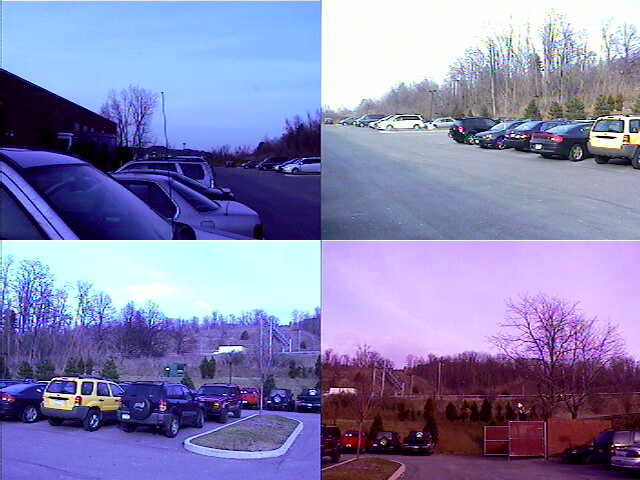
\includegraphics[width=.8\textwidth]{LenelExample}
\caption{Lenel Parking Lot Example}
\label{LenelExample}
\end{figure}

\end{center}
\end{frame}


% INTRODUCTION 002
\begin{frame}[c]{\sc Introduction}
\begin{center}

\begin{figure}[!h]
\centering
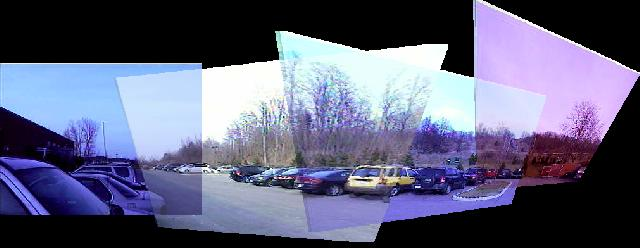
\includegraphics[width=.9\textwidth]{LenelExampleStitched}
\caption{Stitched Images from Lenel Parking Lot Example}
\label{LenelExampleStitched}
\end{figure}

\end{center}
\end{frame}



%%%%%%%%%%%%%%%%%%%%%%%%%%%%%%%%%%%%%%%%%%%%%%%%%%%%%%%%%%%%%%%%%%%%%%%%%%%%%%%
% OVERVIEW
\begin{frame}[t]{\sc Overview}
\begin{center}
We begin by looking at the current fields of research and what theoretical developments must be understood in continuing these areas of research, then go over the foundational work done by the WFMI algorithm, and propose future areas of research and application.
\end{center}

\begin{itemize}
\item Mutual Information
\item Image Registration
\item Motion Estimation
\item Depth Determination
\item The WFMI Algorithm
\item Review and Proposal
\end{itemize}
\end{frame}




%%%%%%%%%%%%%%%%%%%%%%%%%%%%%%%%%%%%%%%%%%%%%%%%%%%%%%%%%%%%%%%%%%%%%%%%%%%%%%%
% MUTUAL INFORMATION 001
\begin{frame}[c]{\sc Mutual Information}

\begin{figure}
\centering
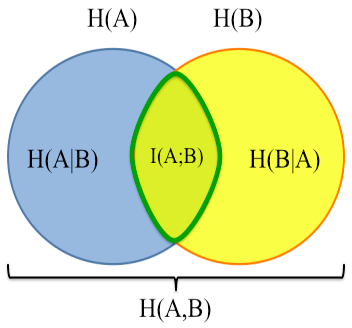
\includegraphics[height=.7\textheight]{informationTheory}
\caption{Venn diagram of key measures in Information Theory}
\label{infoTheory}
\end{figure}


\end{frame}


% MUTUAL INFORMATION 002
\begin{frame}[c]{\sc Mutual Information}

\textbf{Entropy}: The expected value of the self-information, thought of as the measure of randomness in the image data.
\begin{equation}
\label{entropy}
    H(A) = \sum_{i}{p_{A}(a_{i}) \log_{n}{\left(p_{A}(a_{i})\right)}}
\end{equation}

\vfill

\textbf{Probability Mass Function (PMF)}: The distribution of the random data in an image, shown as the normalized histogram of the image data.
\begin{equation}
\label{PMF}
    p_{A}(\bf{a})=h_{A}(\bf{a}) \cdot \left(\sum_{i}{h_{A}(a_{i})} \right)^{-1} = \frac{h_{A}(\bf{a})}{\mathfrak{m}\cdot\mathfrak{n}}
\end{equation}


\end{frame}


% MUTUAL INFORMATION 003
\begin{frame}[c]{\sc Mutual Information}

\textbf{Mutual Information}: The expected value of the ratio of the joint distribution to the product of the marginal distributions. This is thought of as the amount of knowledge that can be obtained about an image from knowledge about another image.
\begin{equation}
\label{MutualInformation}
    I(A;B) = \sum_{j}{\sum_{i}{p_{AB}(a_{i},b_{j}) \log_{2}{\left( \frac{p_{AB}(a_{i},b_{j})}{p_{A}(a_{i})p_{B}(b_{j})}\right)}}}
\end{equation}

\vfill

\textbf{Normalized Mutual Information}: Also known as Symmetric Uncertainty.
\begin{equation}
\label{NormalizedMutualInformation}
    I_{N}(A;B) = \left( \frac{2}{H(A) + H(B)}\right) \cdot I(A;B)
\end{equation}

\end{frame}




%%%%%%%%%%%%%%%%%%%%%%%%%%%%%%%%%%%%%%%%%%%%%%%%%%%%%%%%%%%%%%%%%%%%%%%%%%%%%%%
% IMAGE REGISTRATION 001
\begin{frame}[c]{\sc Image Registration}

\begin{figure}
\centering
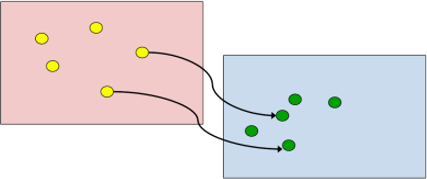
\includegraphics[width=.95\textwidth]{imageRegistration}
\caption{Basic Idea of Image Registration}
\label{imageRegistration}
\end{figure}

\end{frame}



% IMAGE REGISTRATION 002
\begin{frame}[c]{\sc Finding Homographies}

\textbf{Affine Homography}:
\begin{equation}
\label{AffineHomographySolve}
\begin{bmatrix}\sfrac{\hat{x}}{1}\\\sfrac{\hat{y}}{1}\\1\end{bmatrix}=\begin{bmatrix}\hat{x}\\\hat{y}\\1\end{bmatrix}=\begin{bmatrix}a_{11}&a_{12}&a_{13}\\a_{21}&a_{22}&a_{23}\\0&0&1\end{bmatrix}\begin{bmatrix}x\\y\\1\end{bmatrix}
\end{equation}

\vfill

\textbf{Projective Homography}:
\begin{equation}
\label{ProjectiveHomographySolve}
\begin{bmatrix}\sfrac{\hat{x}}{\hat{z}}\\\sfrac{\hat{y}}{\hat{z}}\\1\end{bmatrix}=\begin{bmatrix}\hat{x}\\\hat{y}\\\hat{z}\end{bmatrix}=\begin{bmatrix}p_{11}&p_{12}&p_{13}\\p_{21}&p_{22}&p_{23}\\p_{31}&p_{32}&1\end{bmatrix}\begin{bmatrix}x\\y\\1\end{bmatrix}
\end{equation}

\end{frame}



% IMAGE REGISTRATION 003
\begin{frame}[t]{\sc Solving for Homographies}

\textbf{Direct Linear Transformation}:

\begin{center}
Method for solving for Homography relating pixels between two images.

\begin{equation}
\label{DLT}
    A=\hat{\bf{x}}_{i} \times H \bf{x}_{i}=0
\end{equation}

\begin{equation}
\label{DLTSVD}
    A=U \Sigma V^{H}
\end{equation}

\begin{equation}
\label{SVD}
    \Sigma = \begin{bmatrix}\sigma_{1}&0&0&0&\cdots&0 \\ 0&\sigma_{2}&0&0&\cdots&0 \\ 0&0&\sigma_{3}&0&\cdots&0 \\ &&&\ddots&& \end{bmatrix}
\end{equation}

\end{center}

\end{frame}


%%%%%%%%%%%%%%%%%%%%%%%%%%%%%%%%%%%%%%%%%%%%%%%%%%%%%%%%%%%%%%%%%%%%%%%%%%%%%%%
% MOTION ESTIMATION

% MOTION ESTIMATION 001
\begin{frame}[c]{\sc Motion in Video}

\begin{figure}[!h]
\centering
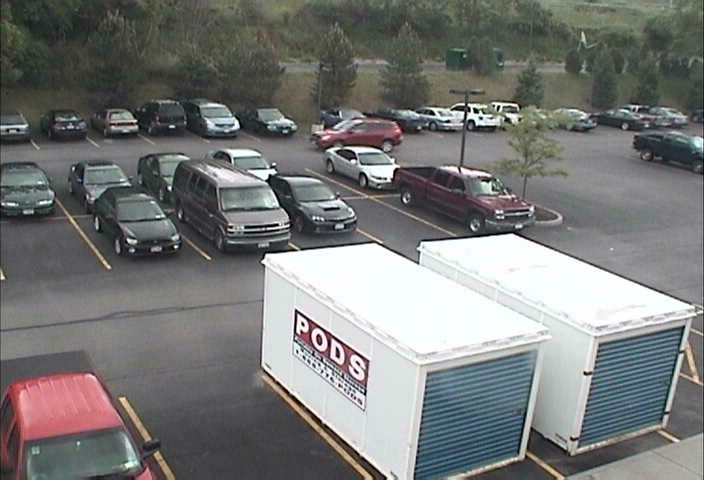
\includegraphics[width=.9\textwidth]{Lenel010L(555)}
\caption{Lenel Parking Lot, Frame 555}
\label{Lenel555}
\end{figure}

\end{frame}

% MOTION ESTIMATION 001
\begin{frame}[c]{\sc Motion in Video}

\begin{figure}[!h]
\centering
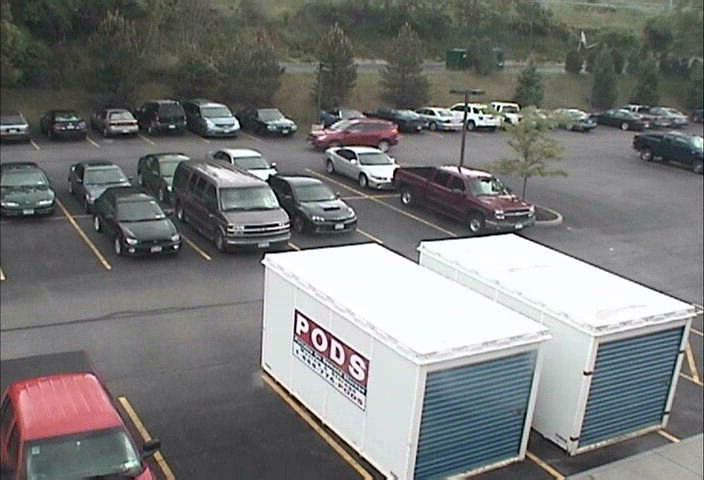
\includegraphics[width=.9\textwidth]{Lenel010L(556)}
\caption{Lenel Parking Lot, Frame 556}
\label{Lenel556}
\end{figure}

\end{frame}

% MOTION ESTIMATION 001
\begin{frame}[c]{\sc Motion in Video}

\begin{figure}[!h]
\centering
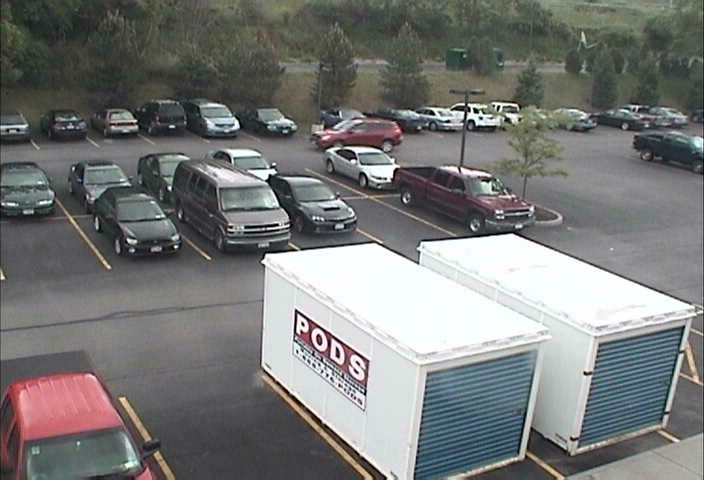
\includegraphics[width=.9\textwidth]{Lenel010L(555)}
\caption{Lenel Parking Lot, Frame 555}
\label{Lenel555s}
\end{figure}

\end{frame}

% MOTION ESTIMATION 001
\begin{frame}[c]{\sc Motion in Video}

\begin{figure}[!h]
\centering
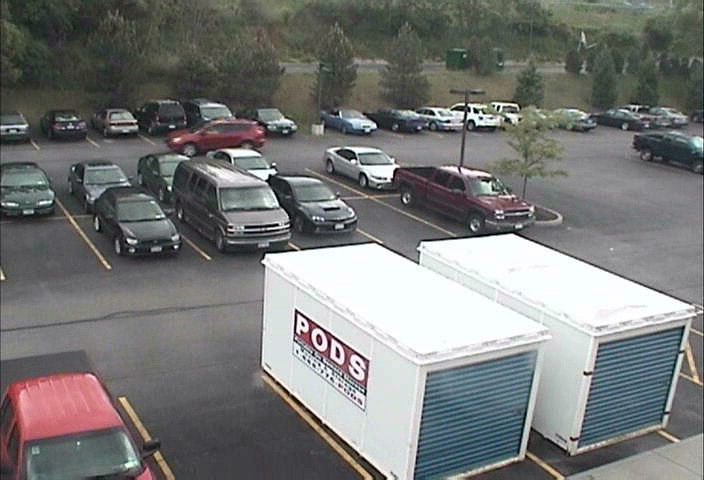
\includegraphics[width=.9\textwidth]{Lenel010L(590)}
\caption{Lenel Parking Lot, Frame 590}
\label{Lenel590}
\end{figure}

\end{frame}


% MOTION ESTIMATION 002
\begin{frame}[c]{\sc Motion Estimation}

\begin{itemize}
\item Optical Flow Constraint
\item Gibbs Random Fields
\item Video Frame Registration
\item Gradient Descent Algorithms
\end{itemize}

\end{frame}





%%%%%%%%%%%%%%%%%%%%%%%%%%%%%%%%%%%%%%%%%%%%%%%%%%%%%%%%%%%%%%%%%%%%%%%%%%%%%%%
% DEPTH DETERMINATION

% DEPTH DETERMINATION 001
\begin{frame}[t]{\sc Depth Determination}

\begin{figure}[!h]
\centering
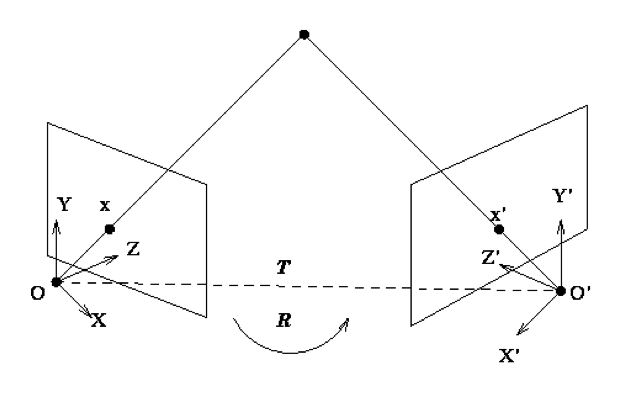
\includegraphics[width=.9\textwidth]{CameraGeometry}
\caption{Multiple View Camera Geometry (Image from \cite{Hartley2003})}
\label{CameraGeometry}
\end{figure}

\end{frame}


%%%%%%%%%%%%%%%%%%%%%%%%%%%%%%%%%%%%%%%%%%%%%%%%%%%%%%%%%%%%%%%%%%%%%%%%%%%%%%%
% WFMI ALGORITHM

% ALGORITHM STEPS
\begin{frame}[c]{\sc WFMI Algorithm}
\begin{itemize}
\item Two Color Images
\item Color Gradient Maps
\item Histogram-Based Quantization of Color Gradients
\item Assume Image B as Reference, Transform Image A
\item Create Mutual Information Map through Translation Search
\item Weight the Mutual Information Map
\item Laplacian Filter the Weighted Mutual Information Map
\item Store Peak Value and Location
\item Move to next Transformation and Find next Peak
\item Take Maximum Peak and Transform Image A
\item Blend Images A and B
\end{itemize}
\end{frame}



\begin{frame}[c]{\sc WFMI Algorithm}

\begin{figure}[!h]
\centering
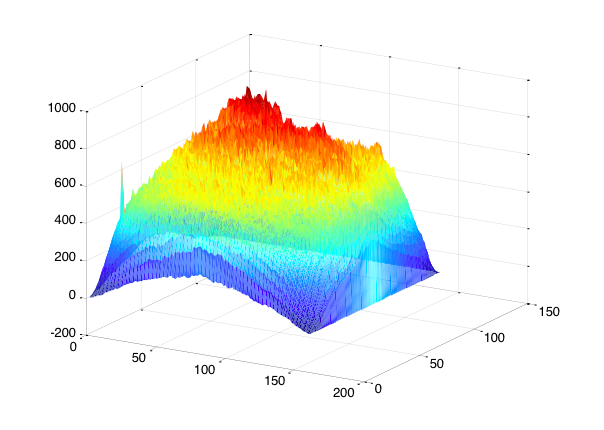
\includegraphics[height=.7\textheight]{MutualInformationMap}
\caption{Mutual Information Map from Translation Search}
\label{MutualInformationMap}
\end{figure}

\end{frame}


\begin{frame}[c]{\sc WFMI Algorithm}

\begin{figure}[!h]
\centering
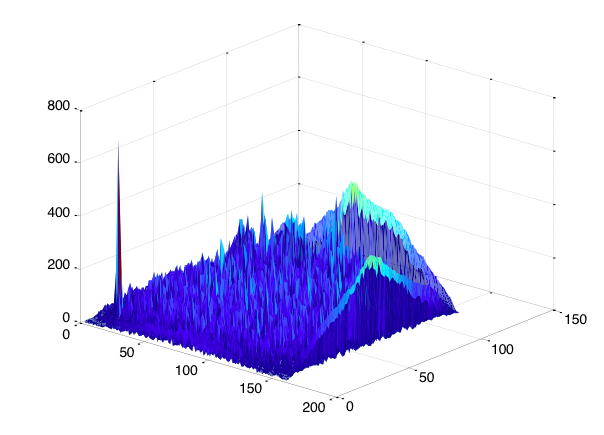
\includegraphics[height=.7\textheight]{FilteredMutualInformationMap}
\caption{Weighted and Filtered Mutual Information Map}
\label{FilteredMap}
\end{figure}

\end{frame}





\begin{frame}[c]{\sc WFMI Algorithm}

\begin{figure}[!h]
\centering
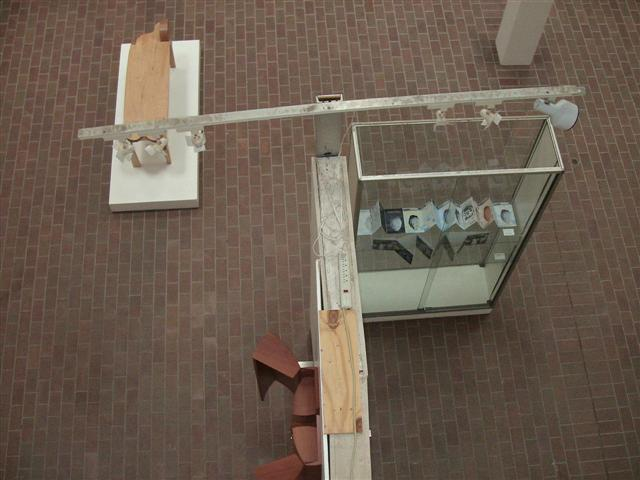
\includegraphics[height=.7\textheight]{AGS4L005}
\caption{Original Image}
\label{ArtGalleryOriginal}
\end{figure}

\end{frame}


\begin{frame}[c]{\sc WFMI Algorithm}

\begin{figure}[!h]
\centering
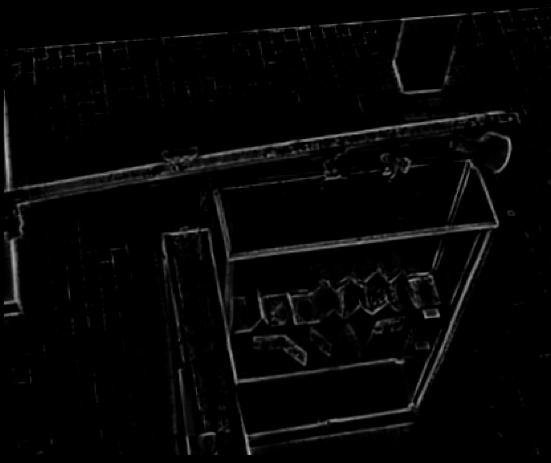
\includegraphics[height=.7\textheight]{ColorEdges}
\caption{Color Gradient Map \cite{Lee1991}}
\label{ArtGalleryGradient}
\end{figure}

\end{frame}


\begin{frame}[c]{\sc WFMI Algorithm}

\begin{figure}[!h]
\centering
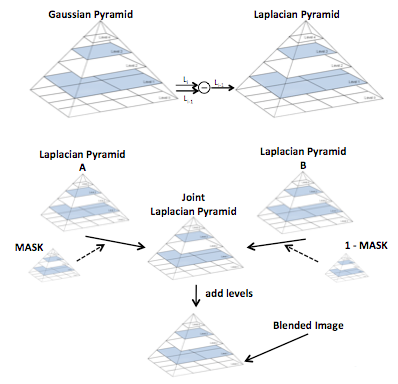
\includegraphics[height=.7\textheight]{MultiresolutionSpline}
\caption{Multiresolution Spline Blending \cite{Burt1983}}
\label{MultiresolutionSpline}
\end{figure}

\end{frame}







%%%%%%%%%%%%%%%%%%%%%%%%%%%%%%%%%%%%%%%%%%%%%%%%%%%%%%%%%%%%%%%%%%%%%%%%%%%%%%%
% WFMI RESULTS 001
\begin{frame}[c]{\sc Affine Frames}

\begin{figure}[!h]
\centering
\subfigure{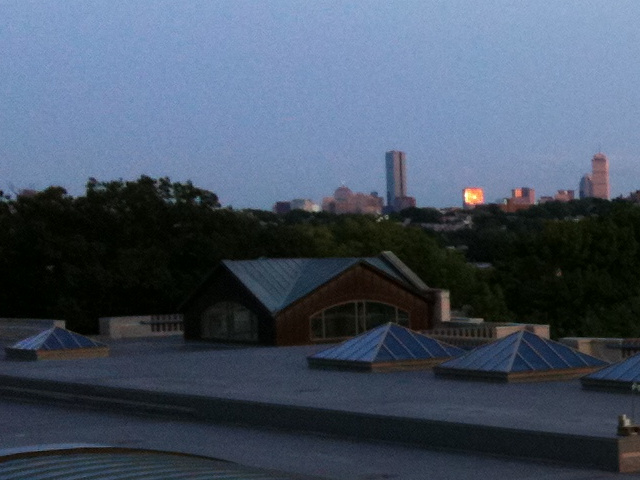
\includegraphics[width=.48\textwidth]{RooftopL001} \label{RooftopL}}
\subfigure{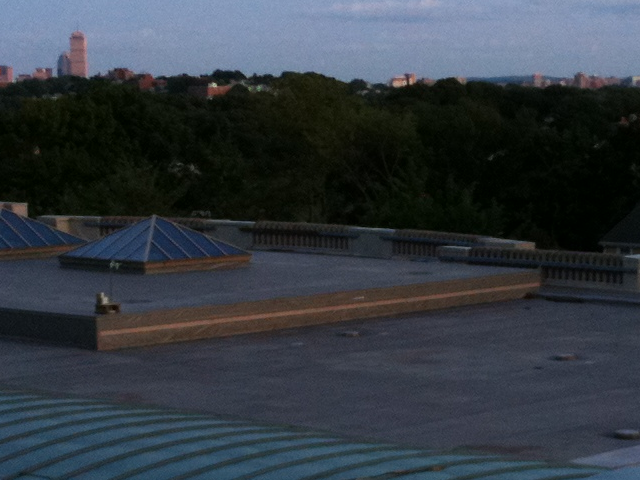
\includegraphics[width=.48\textwidth]{RooftopR001} \label{RooftopR}}
\caption{Rooftop Scene (a) Left View, (b) Right View}
\label{RooftopImages}
\end{figure}

\end{frame}

% WFMI RESULTS 001
\begin{frame}[c]{\sc Affine Panorama}

\begin{figure}[!h]
\centering
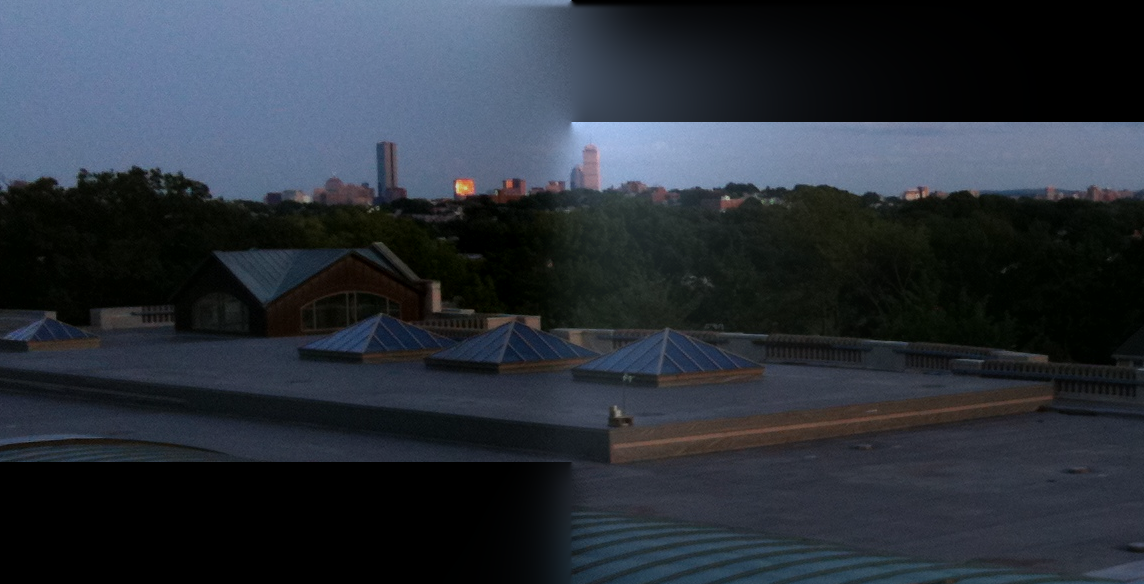
\includegraphics[width=1\textwidth]{RooftopSP001001}
\caption{Rooftop Views Blended}
\label{RooftopStitched}
\end{figure}

\end{frame}


% WFMI RESULTS 002
\begin{frame}[c]{\sc Near Affine Frames}

\begin{figure}[!h]
\centering
\subfigure{ 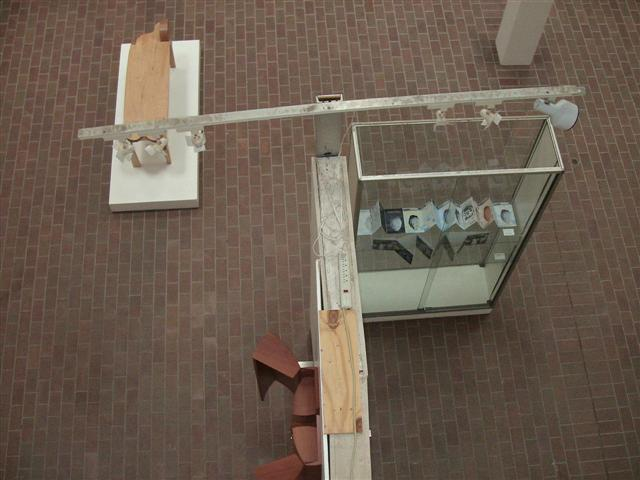
\includegraphics[width=.4\textwidth]{AGS4L005} \label{ArtGallery4L} }
\subfigure{ 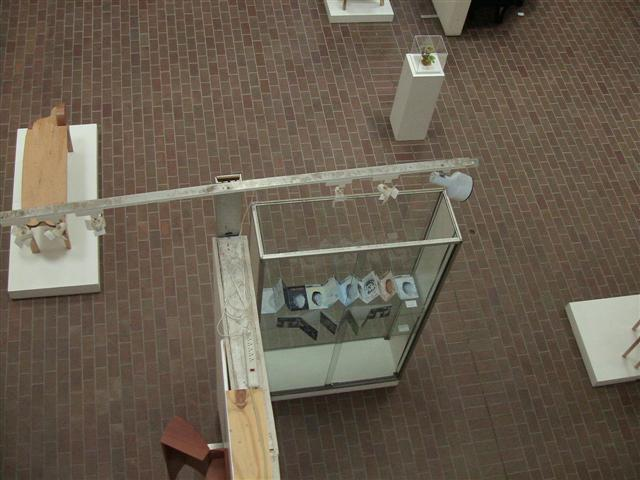
\includegraphics[width=.4\textwidth]{AGS4R005} \label{ArtGallery4R} }
\caption{Art Gallery 04 Scene (a) Left View, (b) Right View}
\label{ArtGallery4Images}
\end{figure}

\end{frame}

% WFMI RESULTS 002
\begin{frame}[c]{\sc Near Affine Panorama}

\begin{figure}[!h]
\centering
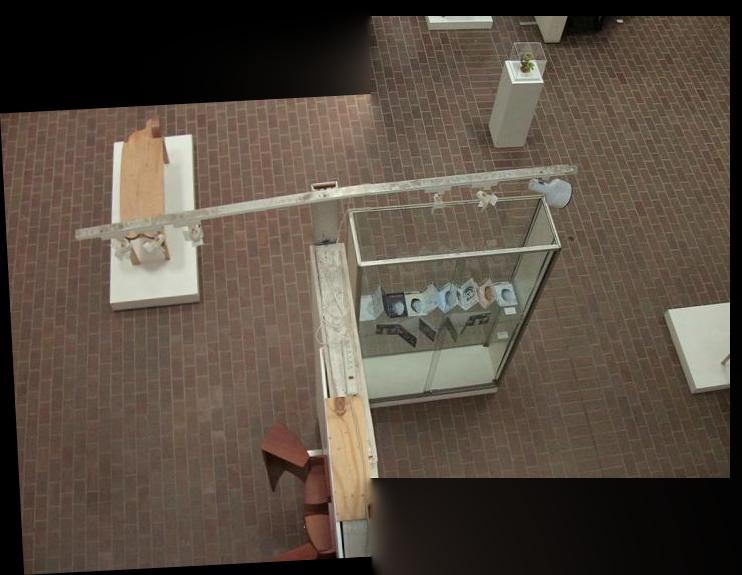
\includegraphics[width=.8\textwidth]{AGS4SP005005}
\caption{Art Gallery 04 Views Blended}
\label{ArtGallery4Stitched}
\end{figure}

\end{frame}


% WFMI RESULTS 003
\begin{frame}[c]{\sc Complex Projective Frames}

\begin{figure}[!h]
\centering
\subfigure[]{ 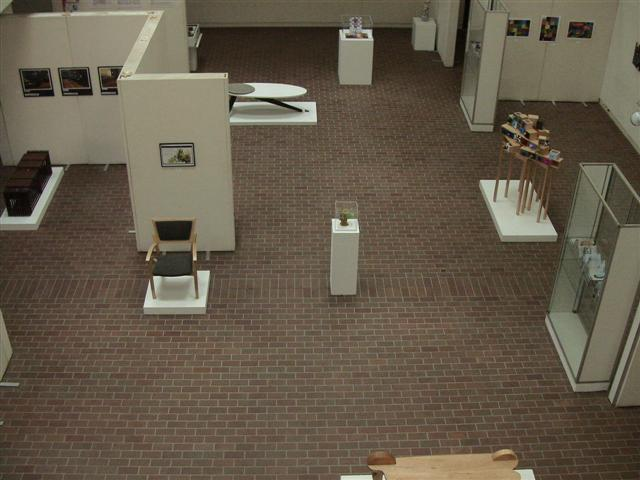
\includegraphics[width=.45\textwidth]{AGS1L001} \label{ArtGallery1L} }
\subfigure[]{ 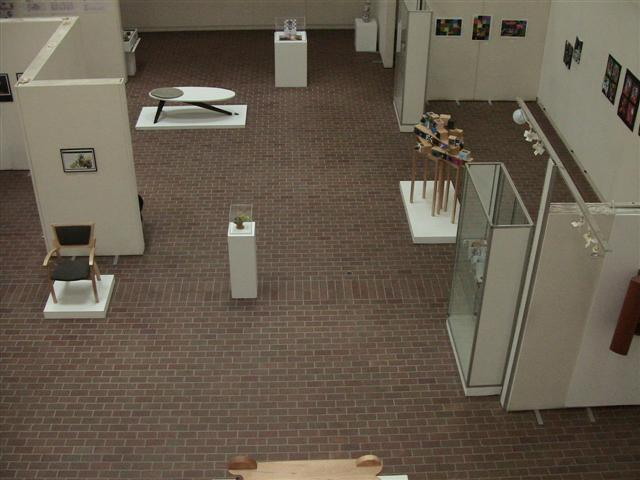
\includegraphics[width=.45\textwidth]{AGS1R001} \label{ArtGallery1R} }
\caption{Art Gallery Scene 01 (a) Left View, (b) Right View}
\label{ArtGallery1Images}
\end{figure}

\end{frame}

% WFMI RESULTS 003
\begin{frame}[c]{\sc Complex Projective Panorama}

\begin{figure}[!h]
\centering
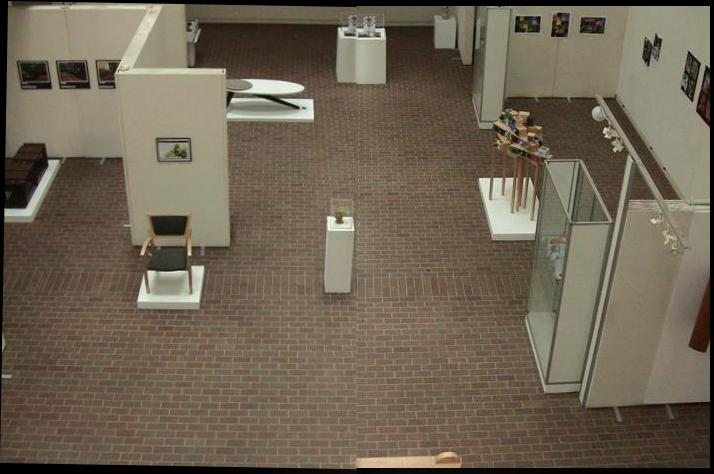
\includegraphics[width=.9\textwidth]{AGS1SP001001}
\caption{Art Gallery 01 Views Blended}
\label{ArtGallery1Stitched}
\end{figure}

\end{frame}


% WFMI RESULTS 004
\begin{frame}[c]{\sc Complex Projective Frames}

\begin{figure}[!h]
\centering
\subfigure[]{ 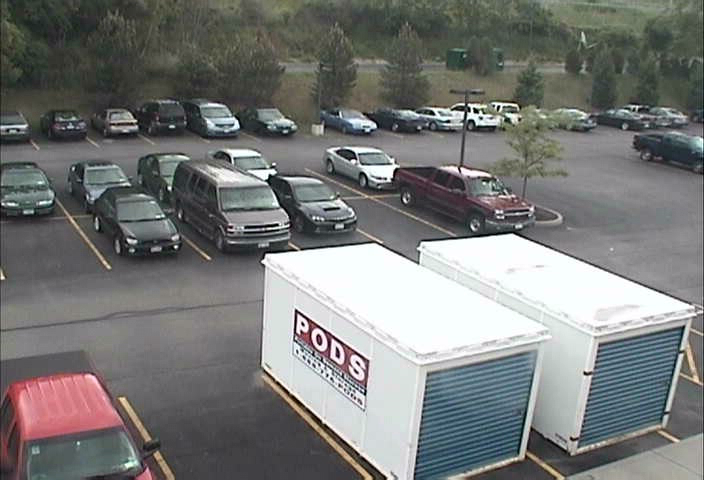
\includegraphics[width=.45\textwidth]{Lenel010L004} \label{Lenel10L} }
\subfigure[]{ 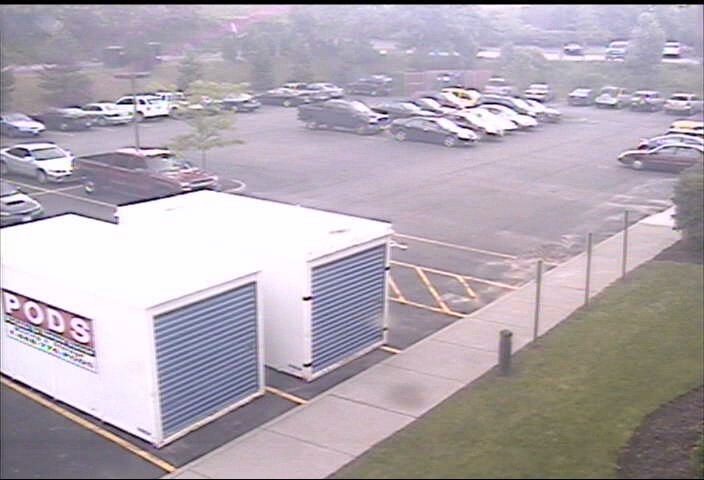
\includegraphics[width=.45\textwidth]{Lenel010R004} \label{Lenel10R} }
\caption{Lenel Back Lot Scene (a) Left View, (b) Right View}
\label{Lenel10Images}
\end{figure}

\end{frame}

% WFMI RESULTS 004
\begin{frame}[c]{\sc Complex Projective Panorama}

\begin{figure}[!h]
\centering
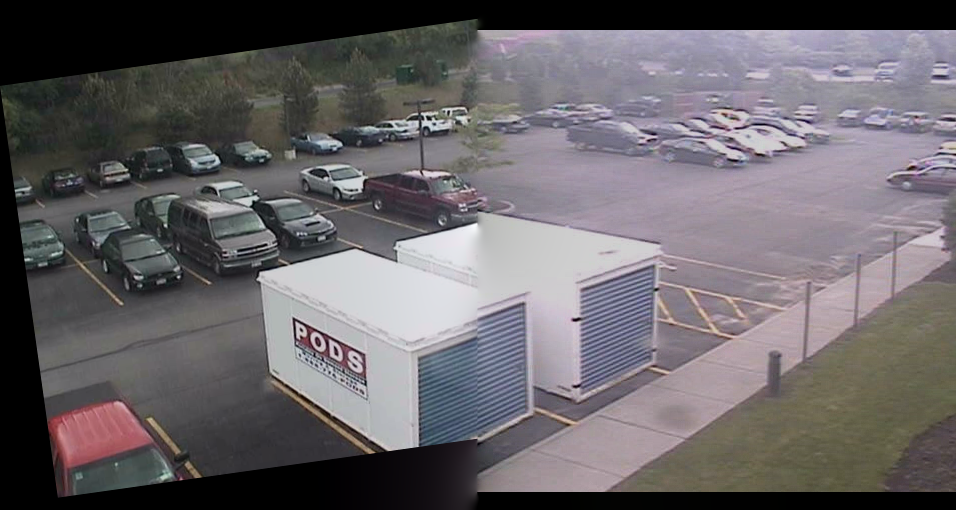
\includegraphics[width=1\textwidth]{Lenel010SP001}
\caption{Lenel Back Lot Views Blended}
\label{Lenel10Stitched}
\end{figure}

\end{frame}



%%%%%%%%%%%%%%%%%%%%%%%%%%%%%%%%%%%%%%%%%%%%%%%%%%%%%%%%%%%%%%%%%%%%%%%%%%%%%%%
% CONCLUSION
\begin{frame}[c]{\sc Conclusion}
\begin{itemize}
\item Novel Application of Mutual Information
\item Realistic Scenes and Practical Concerns
\item Concepts Theoretically Extensible to Motion Estimation
\item Concepts Theoretically Extensible to Depth Determination
\item Not well-worn Research Territory
\end{itemize}
\end{frame}



%%%%%%%%%%%%%%%%%%%%%%%%%%%%%%%%%%%%%%%%%%%%%%%%%%%%%%%%%%%%%%%%%%%%%%%%%%%%%%%
% REFERENCES
\begin{frame}[allowframebreaks]{\sc References}
\tiny
\bibliography{../LaTeX_Thesis/TommyKeane_MS_Thesis_Bibliography}
\nocite{*}
\end{frame}

%%%%%%%%%%%%%%%%%%%%%%%%%%%%%%%%%%%%%%%%%%%%%%%%%%%%%%%%%%%%%%%%%%%%%%%%%%%%%%%
% END OF DOCUMENT
%%%%%%%%%%%%%%%%%%%%%%%%%%%%%%%%%%%%%%%%%%%%%%%%%%%%%%%%%%%%%%%%%%%%%%%%%%%%%%%
\end{document}
